\chapter{技术背景与实验平台}
\label{chapter:chapter2}
本文主要针对Android平台上卷积神经网络的前向推断过程进行能效优化的研究,故而本章首先会对研究工作的主要技术背景进行相关介绍。由于后面章节都会对不同实现方式的能效进行实验评估,故而本章最后一节详细描述了研究中所使用的能效度量标准和实验平台。\ref{chapter:ch2-1}节介绍了卷积神经网络的基本概念,并对卷积神经网络中的几个基本层进行了详细描述;\ref{chapter:ch2-2}节简要描述了反向传播算法中涉及的梯度下降\cite{bottou2010large}和反向传播过程;\ref{chapter:chapteropencl}节主要介绍了OpenCL异构编程框架的基本概念和三个主要开发优点,并给出了使用OpenCL框架进行程序设计的基本开发流程。\ref{chapter:ch2-4}节给出了本文评估能效的度量标准,并详细介绍了本文所使用的实验平台。

\section{卷积神经网络}
\label{chapter:ch2-1}
卷积神经网络(CNNs)是一种深度前向反馈人工神经网络\cite{schalkoff1997artificial},其主要用来处理二维或更高维度的数据,如图像数据、音频数据等。近年来,在众多研究学者的努力下,卷积神经网络在计算机视觉领域已经取得了许多突破性进展,如高精度图像识别、目标检测等。卷积神经网络中主要采用了一种名为“卷积”的数学运算,它将深度神经网络模型部分层中的通用矩阵乘法替换为卷积操作。

\begin{figure}[htbp]
    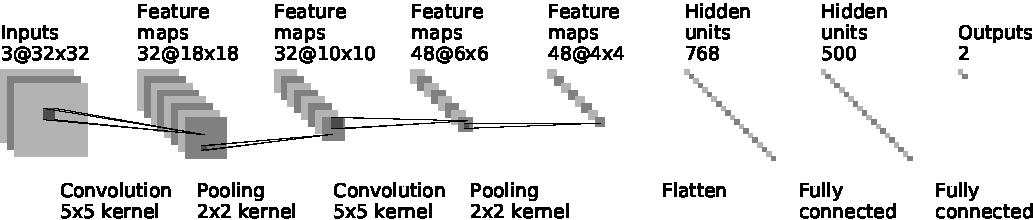
\includegraphics[width=1\textwidth]{figures/convnet_fig_cropped.pdf}
    \caption{卷积神经网络结构示意图 \cite{github.com}}\label{figure:figure1}
\end{figure}

图\ref{figure:figure1}展示了一个卷积神经网络结构案例,其主要由三个基本层组成,即卷积层、池化层和全连接层。简单来说,每一个卷积层通过多个卷积核将前一层低级别特征转换成高级别特征。池化层用于捕捉一些不变性,如对输入图像的平移、旋转或缩放操作不影响卷积处理的输出结果。最后,全连接层通过聚合前面层提取出的高级别特征完成分类任务。除了这三种基本层外,输入数据在经过卷积层或池化层或全连接层之后还可能再附加一层激活层,其主要使得模型具备非线性,以解决非线性分类等问题。接下来的章节将详细描述这些层的含义与作用。

\subsection{卷积层}
\subsubsection{卷积操作}
卷积层从字面上来看必定执行卷积操作,其主要通过将多个滤波器作用在输入图像上完成不同特征的提取。这些滤波器被称作卷积核,且被卷积的图像叫做特征图。下面以图\ref{figure:figure2}表示的图像数据和卷积核为例详细介绍卷积操作的整个过程。

\begin{figure}[htbp]
    \begin{center}
    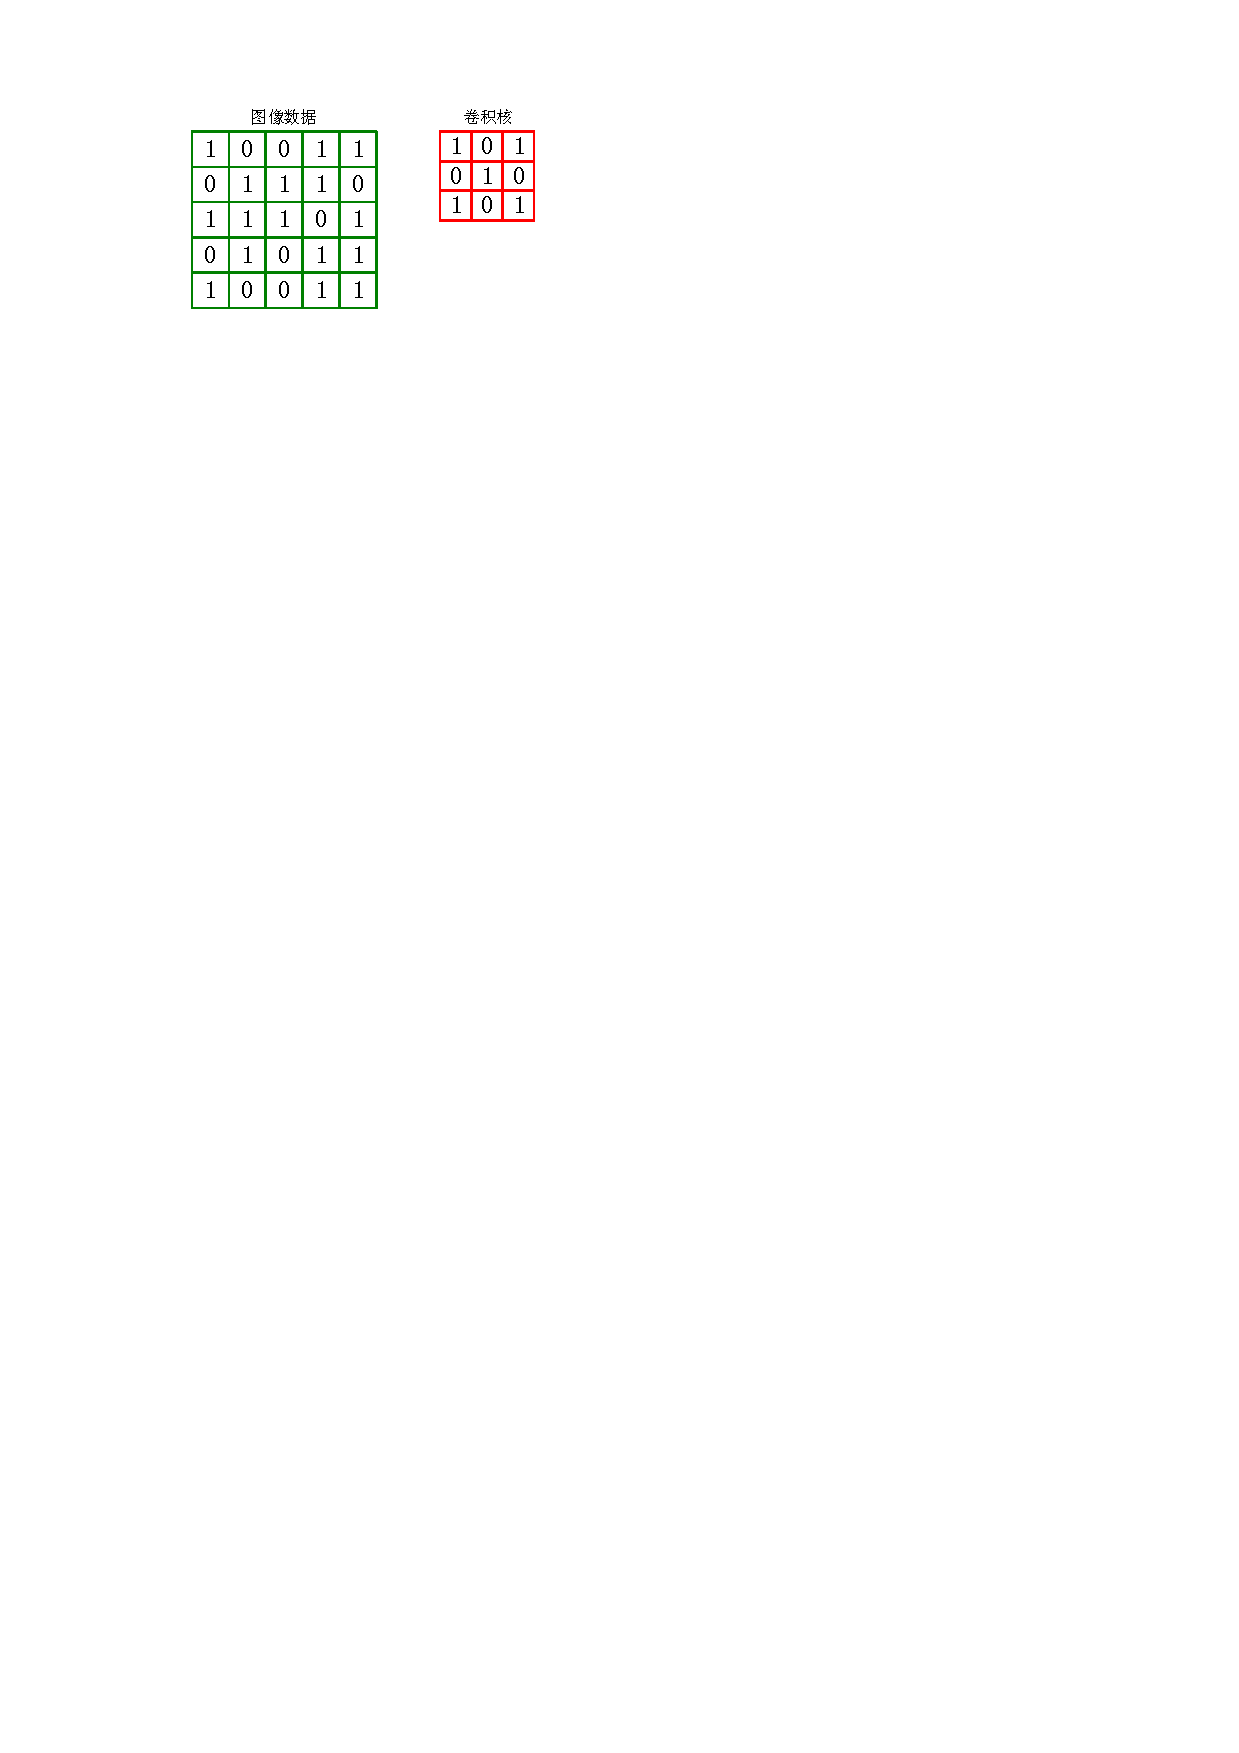
\includegraphics{figures/conv.pdf}
    \end{center}
    \caption{图像数据和卷积核}\label{figure:figure2}
\end{figure}


如图\ref{figure:figure3}所示,卷积核沿着图像从左到右、从上到下按一定步长滑过,并返回卷积核内区域图像像素值与卷积核对应值的乘积之和。通过改变卷积核的值,卷积操作就可以提取到输入图像的不同种类特征。例如,一个中间值为8而其他所有值均为-1的3$\times$3卷积核可以提取图像的边缘特征,因为它强调了颜色的差异;而一个包含所有值均为0.1的3$\times$3卷积核会使得图像变得模糊不清,因为它降低了原始图像像素值。卷积神经网络的强大之处在于卷积层的卷积核权值不需要进行手工设计。卷积神经网络一经初始化后,其自身就可以通过一定的学习算法学习到合适的卷积核权重值。

\begin{figure}[htbp]
    \begin{center}
    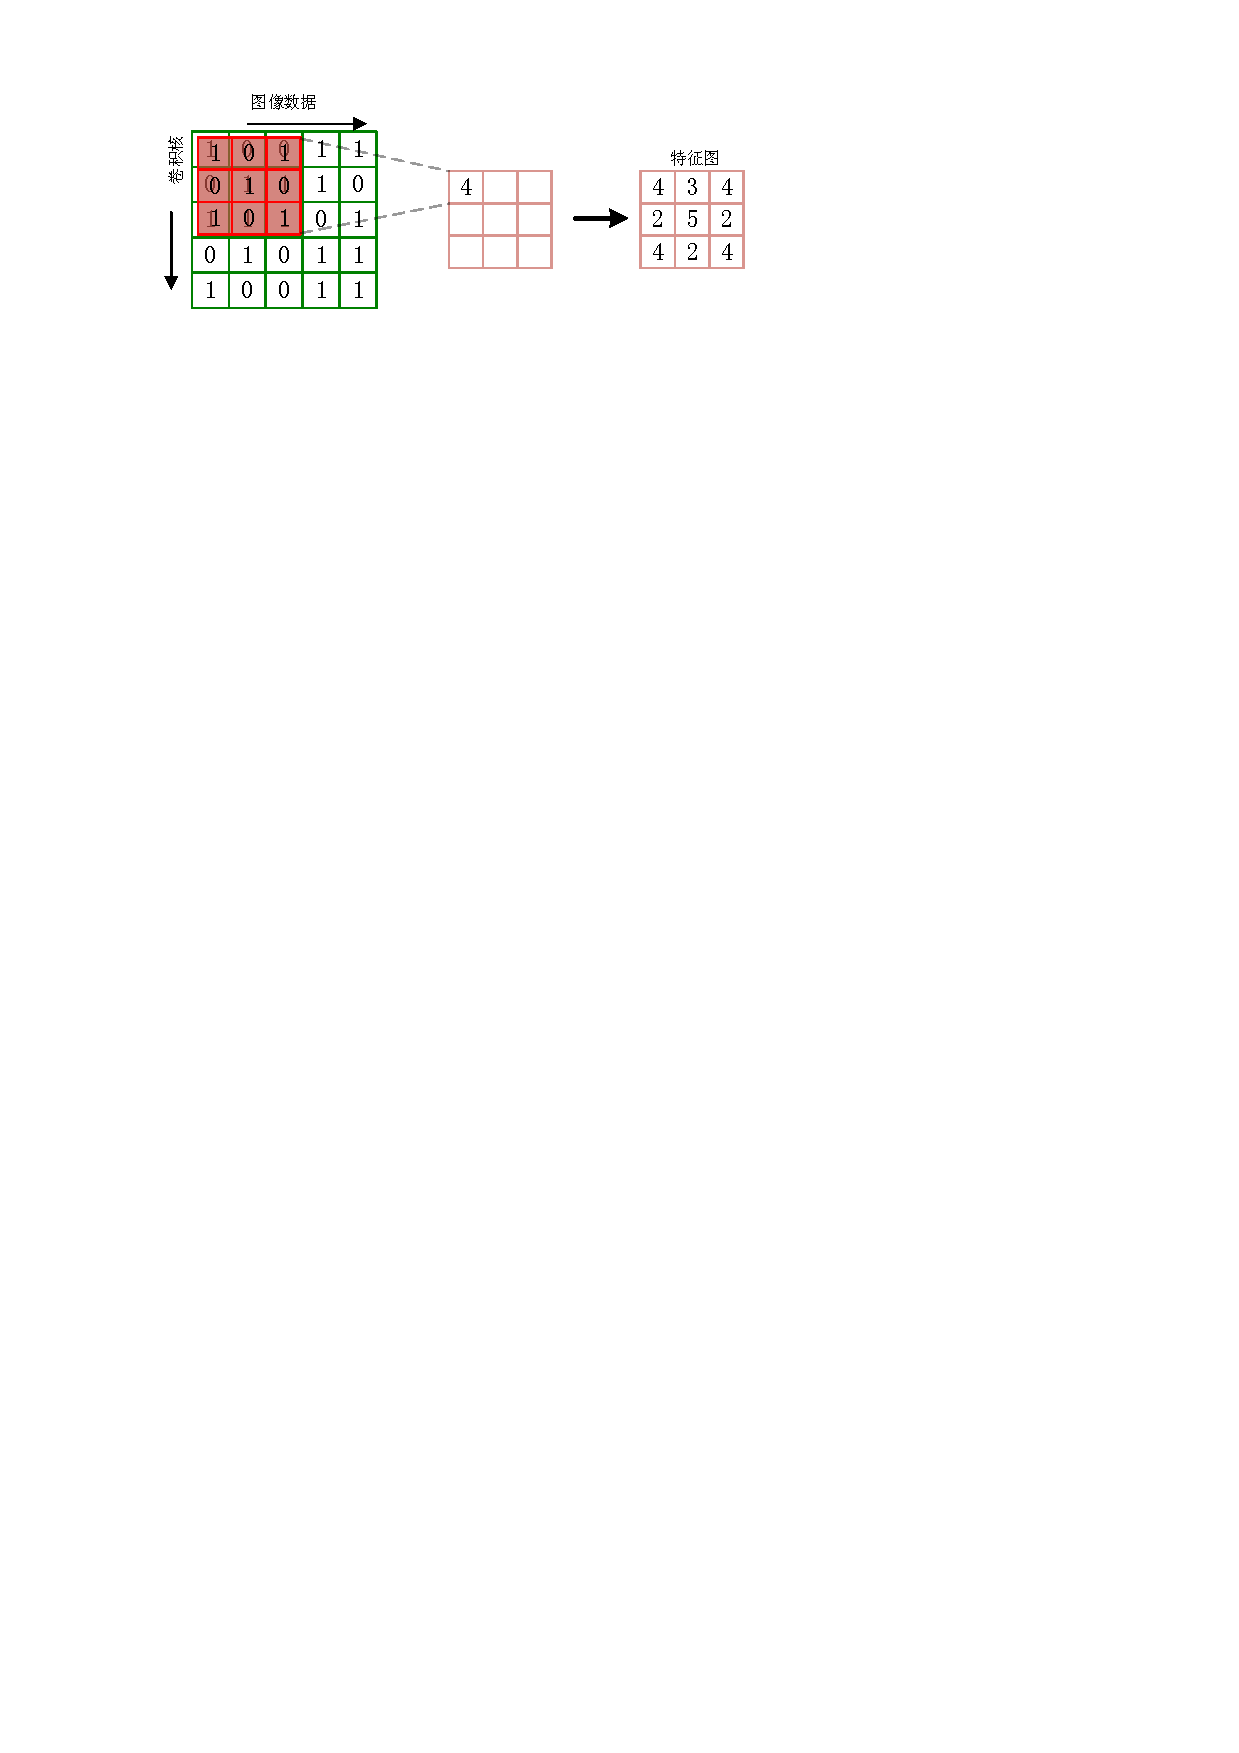
\includegraphics{figures/conv_process.pdf}
    \caption{卷积过程示意图}\label{figure:figure3}
    \end{center}
\end{figure}

\subsubsection{卷积的动机}
带有卷积层的神经网络之所以可得到很高的预测精度,是因为卷积操作利用了三个重要的思想:稀疏交互、参数共享和等变化表示。通过这三个思想,卷积很好地模拟了人类视觉上的局部感受野。下面详述这三个重要思想:

\begin{itemize}
  \item \textbf{稀疏交互}:传统的神经网络层通过一个将每一输入与每一输出相连接的矩阵参数与输入数据进行矩阵乘法运算来得到该层的输出结果。这意味着每一个输出节点与每一个输入节点都是相交互的。然而,卷积神经网络输入与输出之间的连接是稀疏的。换言之,它通过使用许多远小于输入数据尺寸的卷积核将输入节点与输出节点进行连接。例如,在处理一张图像时,输入图像可能拥有成千上百万的像素,但是我们可以使用一个每次只覆盖几十个像素点的卷积核来检测出小的、有意义的特征(如图像边沿等)。这种稀疏连接方式大大降低了卷积模型的权重存储占用。
  \item  \textbf{参数共享}:这意味着对于模型中不同的功能单元可以使用相同的参数。传统神经网络权重矩阵中的每一个元素在计算输出节点时都只会被使用一次。而在卷积神经网络中,卷积核的每一个元素在输入的每一个位置上都会被使用。这依赖于一个合理的假设:如果一块特征的计算在某个空间位置上是有用的,那么它在其他位置上的计算也应该是有用的。
  \item \textbf{等变化表示}:卷积操作的参数共享进一步为卷积网络附加了一个属性,即对不同变换的等变化表示。如果对一个函数的输入施加了某种变换,其输出也会响应相同的改变,那么该函数就是等变化的。特别地,一个函数$f(x)$是等变化的当且仅当$f(g(x))=g(f(x))$。对于卷积来说,如果$g$是对输入进行的任意一种平移变换,那么卷积函数对$g$来说就是等变化的。然而,卷积对于一些其他的变换(如缩放、旋转等)并不是自然等变化的,因此还需要其他的数学机制去处理这些类型的变换。
\end{itemize}

\subsection{池化层}
\label{chapter:chapter2-1-2}
与卷积层相比,池化层就相对比较简单。池化层并不直接参与训练学习,其仅仅是对卷积层传来的图像进行非线性下采样操作。最大池化(max pooling)是目前所有非线性池化操作中最为常用的。它将输入图片划分成一系列非重叠的矩形区域,对于每一个子区域将其最大值作为输出。池化层可以有效地降低数据表示的空间大小、减少网络模型的参数量和计算量,因此它也可以控制过拟合。在一个CNN模型结构中,池化层通常被周期性的插入到紧挨卷积层之后。另外,池化操作也提供了另外一种形式的平移不变性。

池化层独立地作用在输入数据的每一个通道上以调整它的空间尺寸。如图\ref{figure:figure4}所示,使用$2\times2$的滤波器在输入数据的每一个通道上沿宽和高两个方向进行步长为2的下采样操作是池化层中一个最为常用的形式,其可以丢弃$75\%$的激活结果。在该示例中,最大化操作一次作用在4个数字上,并将4个数字中的最大值作为其输出结果。经池化操作后,输入数据的深度维度是保持不变的。

\begin{figure}[htbp]
    \begin{center}
    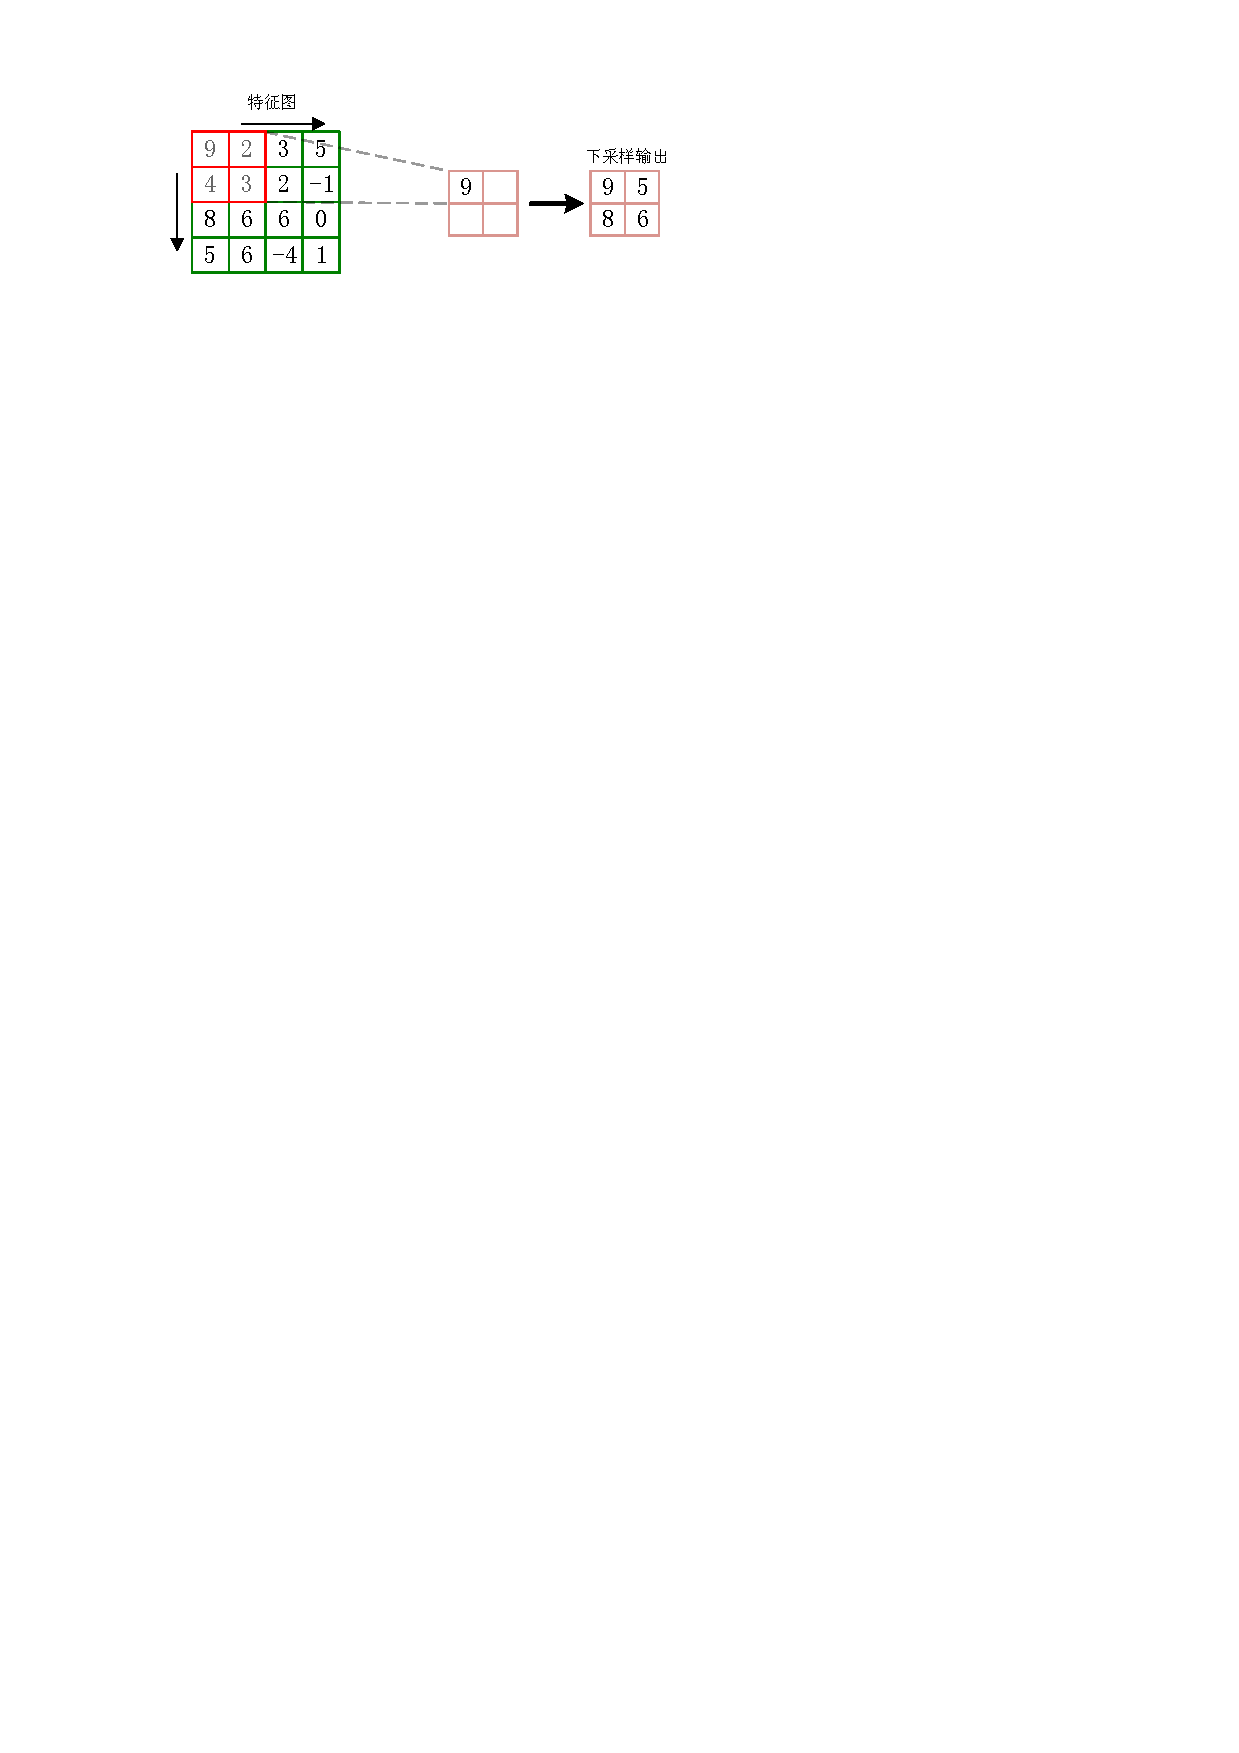
\includegraphics{figures/pool.pdf}
    \end{center}
    \caption{最大池化过程示意图}\label{figure:figure4}
\end{figure}

除了最大池化外,池化单元也可以使用其他函数,如平均池化或L2-正则池化等。平均池化在之前的研究中使用较多,但在近几年越来越多地被最大池化所代替,最大池化已被实践验证下采样效果更佳。

\subsection{全连接层}

在若干个卷积层和池化层之后,更高级别的逻辑分类是由全连接层完成的。如图\ref{figure:figure5}所示,全连接层的神经元与前一层的所有激活值进行全连接,其输出值是由输入神经元与权值矩阵进行内积操作并加上偏置矩阵(如果存在的话)而得到的。

\begin{figure}[htbp]
    \begin{center}
    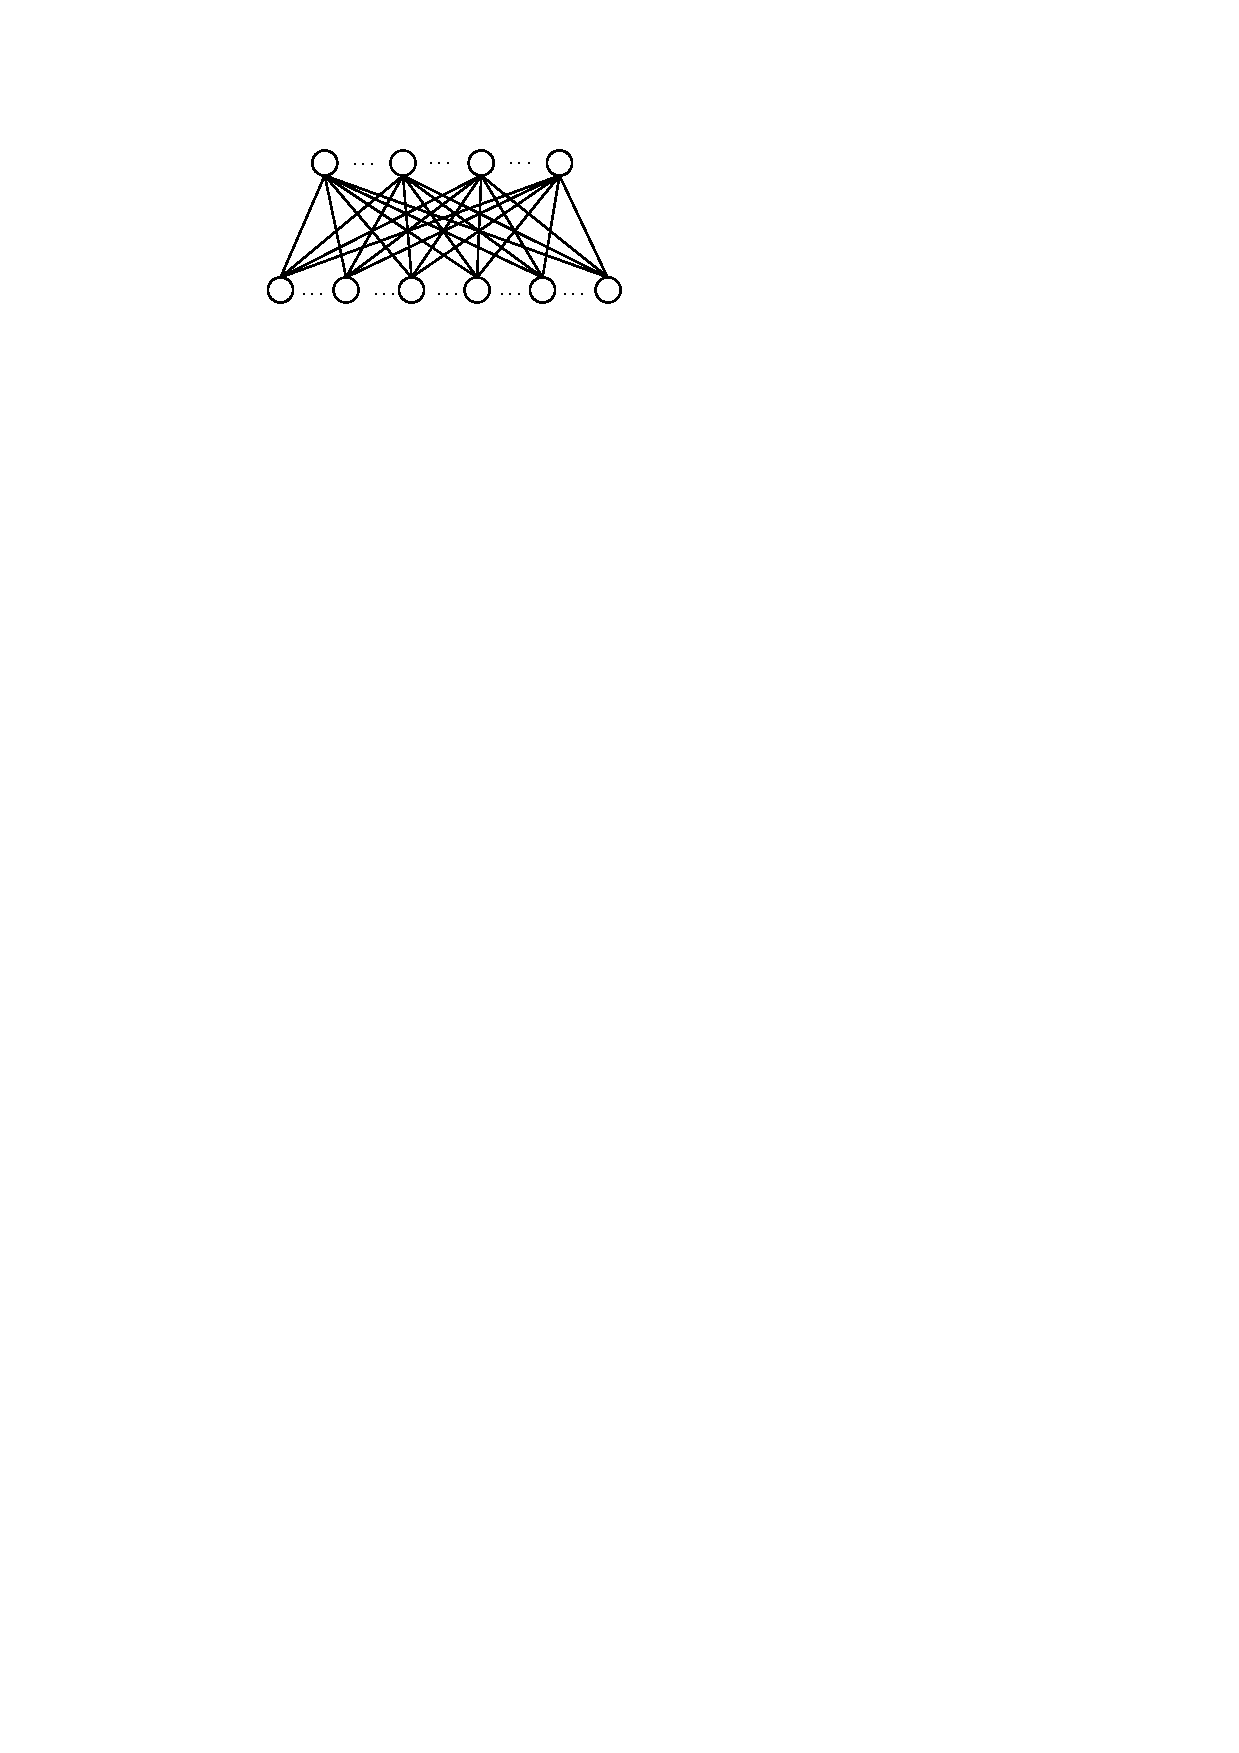
\includegraphics{figures/fc.pdf}
    \end{center}
    \caption{全连接层示意图}\label{figure:figure5}
\end{figure}

\subsection{激活层}
\label{chapter:chapter2-1-4}
激活层主要使用非线性激活函数来增强决策函数和整个网络模型的非线性属性,同时其不会影响卷积层的感受野。Sigmod函数($f(x)=(1+e^{-x})^{-1}$)、Relu函数($f(x)=max(0,x)$)以及双曲正切函数($f(x)=\tanh(x)$)是激活层最为常用的非线性函数,它们的函数图像如图\ref{figure:figure6}所示。其中,Relu函数是近年来被研究人员所青睐的非线性激活函数,因为它不仅更接近生物神经激活函数还可以在一定程度上抑制梯度消失问题的出现,而且相对于其他激活函数,使用Relu函数的模型训练速度会更快。

\begin{figure}[htbp]
    \begin{center}
    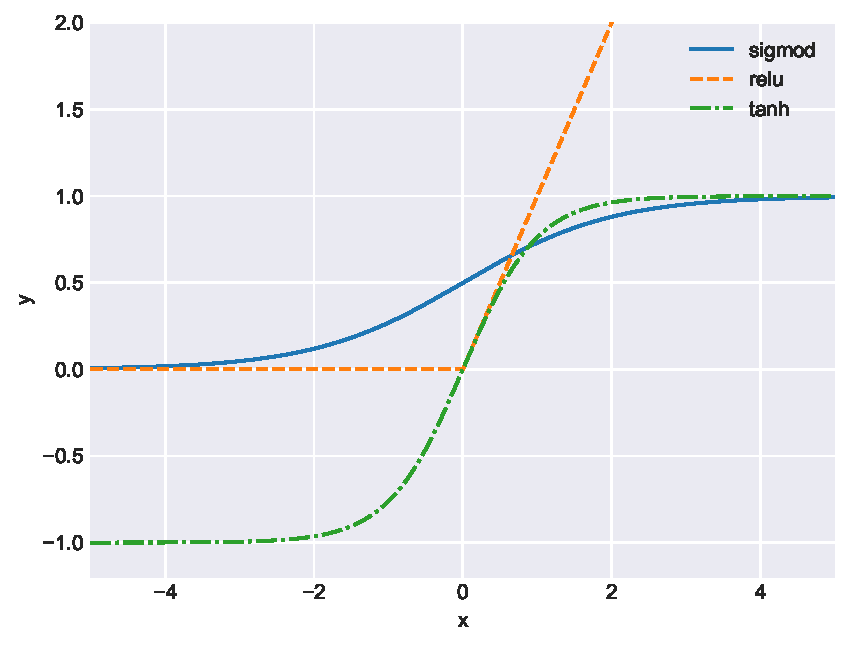
\includegraphics[height=0.4\textwidth]{figures/relu.pdf}
    \end{center}
    \caption{三种非线性激活函数}\label{figure:figure6}
\end{figure}

\section{反向传播算法}
\label{chapter:ch2-2}
在设计好CNN模型的结构之后,利用训练样本和损失函数就可以通过反向传播算法求出CNN模型中的参数矩阵值。反向传播算法是“误差反向传播”的简称,它是目前训练人工神经网络的最重要方法。反向传播算法主要使用梯度下降法求取模型最优权重,即通过预定义的损失函数计算网络模型中所有权重的梯度,并使用这些梯度来更新权值以最小化损失函数。下面首先介绍梯度下降法,然后详细描述反向传播的计算过程。

\subsection{梯度下降}
在机器学习任务中,需要最小化损失函数$L(\theta)$,其中$\theta$是要求解的模型参数。梯度下降法常用来求解这种无约束最优化问题,它是一种迭代方法:选取初值$\theta^0$,不断迭代,更新$\theta$的值,进行损失函数的极小化。梯度下降的迭代公式为$\theta^t=\theta^{t-1}-\alpha L^{'}(\theta^{t-1})$,其详细推导过程描述如下:

\begin{itemize}
  \item 参数更新的迭代公式:$\theta^t=\theta^{t-1}+\Delta\theta$
  \item 将$L(\theta^t)$在$\theta^{t-1}$处进行一阶泰勒展开:
  $$
  L(\theta^t)=L(\theta^{t-1}+\Delta\theta) \\
  \approx L(\theta^{t-1}) + L^{'}(\theta^{t-1})\Delta\theta
  $$
  \item 要使得$L(\theta^t) < L(\theta^{t-1})$,可取:$\Delta\theta=-\alpha L^{'}(\theta^{t-1})$,则:$\theta^t=\theta^{t-1}-\alpha L^{'}(\theta^{t-1})$。此处$\alpha$是步长,一般取一个较小的数值。
\end{itemize}


\subsection{反向传播}

反向传播算法主要使用链式求导法则和梯度下降法将损失函数对于每一层的误差沿层回传以更新每层参数的权重值,其主要包括两个阶段:\textbf{传播}和\textbf{权重更新}。

每一次传播涉及如下步骤:

\begin{itemize}
  \item 通过网络进行前向传播以生成输出值。
  \item 通过损失函数计算损失(即推断误差)。
  \item 沿网络回传所有输出神经元和隐层神经元的增量,即目标值和实际输出值的差值。
\end{itemize}

每一次权值更新必须遵循如下步骤:

\begin{itemize}
  \item 将权重的输出增量和输入激活值相乘以得到权重的梯度。
  \item 一定比重($\alpha$)的权重梯度要从当前权重值中减掉。
\end{itemize}


比重$\alpha$影响着学习速度和学习质量,它也被称为学习率。学习率越高,神经网络的训练速度越快,但是较低的学习率可以使得模型训练更加精确。权重梯度的正负号表示误差是正误差还是负误差,其决定了权重变化方向(增大或减小)。从梯度下降法的推导过程可知,权重必须沿着逆梯度方向增长。上述两个阶段在整个网络模型的学习过程中将不断在不同的批次数据上重复进行直到网络达到预设的性能。

\section{OpenCL异构编程框架}
\label{chapter:chapteropencl}
OpenCL(Open Computing Language)\cite{stone2010opencl}是一个编写跨异构平台可执行程序的编程框架,这些异构平台包括中央处理器(CPUs)、图形显示器(GPUs)、数字信号处理器(DSPs)、现场可编程门阵列(FPGAs)以及一些其他处理器或硬件加速器。OpenCL使用基于C99的编程语言为异构设备编写程序,并使用C/C++语言编写主机程序以控制设备程序在计算设备上的运行。OpenCL为基于任务并行或数据并行的并行计算提供了一个开放的标准接口,并由非盈利技术团队Khronos Group维护。可移植性、标准向量处理和并行编程是吸引开发者选择使用OpenCL编程的三个主要优势。

\subsection{可移植性}
Java因其“一次编译,处处运行”的理念而广受青睐,而OpenCL可能比Java更具可移植性,可以说OpenCL是“一次编写,万物运行”。每一个厂商在提供OpenCL兼容设备的同时也会提供一些工具链去编译OpenCL代码。因此,相同的OpenCL代码只需通过使用各个厂商提供的工具链进行编译便可在不同的硬件设备上运行。这对于常规的高性能计算来说是一个极大的便利,因为在没有OpenCL之前,高性能计算程序设计人员不得不针对不同厂商的硬件设备学习该厂商指定的编程语言。

\subsection{标准向量处理}

标准向量处理是OpenCL的一个巨大优点。与物理或数学上的向量含义不同,这里的向量指的是一种数据结构,其包含多个相同数据类型的元素。在进行向量计算时,对向量中每个元素的操作都是在同一个时钟周期内完成的,可完成这种类型操作的处理器包括超标量处理器或向量处理器等。向量指令通常是由厂商指定且不统一,例如:Intel处理器使用SSE扩展,而英伟达设备使用PTX指令。不同的指令集之间的巨大差异性使得开发人员不能使用标准C/C++进行向量编程,而且标准C/C++语言亦没有原生提供向量数据类型。

然而,程序设计人员可以利用OpenCL一次编写向量例程,并将它们运行在不同的兼容设备上。这些OpenCL程序在不同的平台上会产生不同的编译结果:英伟达的OpenCL编译器将会生成PTX指令,而IBM的编译器会将OpenCL程序编译成AltiVec指令。由此可见,使用OpenCL编写可在不同平台上运行的高性能计算程序是一件省时又省力之事。

\subsection{并行编程}

在OpenCL中,开发人员可使用被称为核函数(\emph{kernels})的数据结构将计算任务分配到不同的处理单元上进行并行执行。一个核函数是一段特殊的函数代码,其可以被一个或多个OpenCL兼容设备执行。核函数被主机应用(\emph{host applications})发送到一个或多个选定的设备上执行。一个主机应用是使用常规C/C++语言编写的程序,其可以运行在用户使用的主机系统上。主机应用不仅可以将核函数分发到从设备(如GPUs)上,还可以让核函数直接在主机应用正在使用的CPU上运行。

主机应用使用一个被称为上下文(\emph{context})的容器管理着与其相连的从设备。图\ref{figure:figure7}显示了主机与核函数以及设备之间的交互。为了创建一个核函数,主机应用从一个被称为核函数容器的程序(\emph{program})中选择一个函数。然后,主机应用设置好该核函数的参数数据并将其分派到一个被称为命令队列的结构中(\emph{command queue})。通过命令队列,主机可以告诉设备需要做的事情。当核函数入列后,设备将执行对应的函数逻辑。

\begin{figure}[htbp]
    \begin{center}
    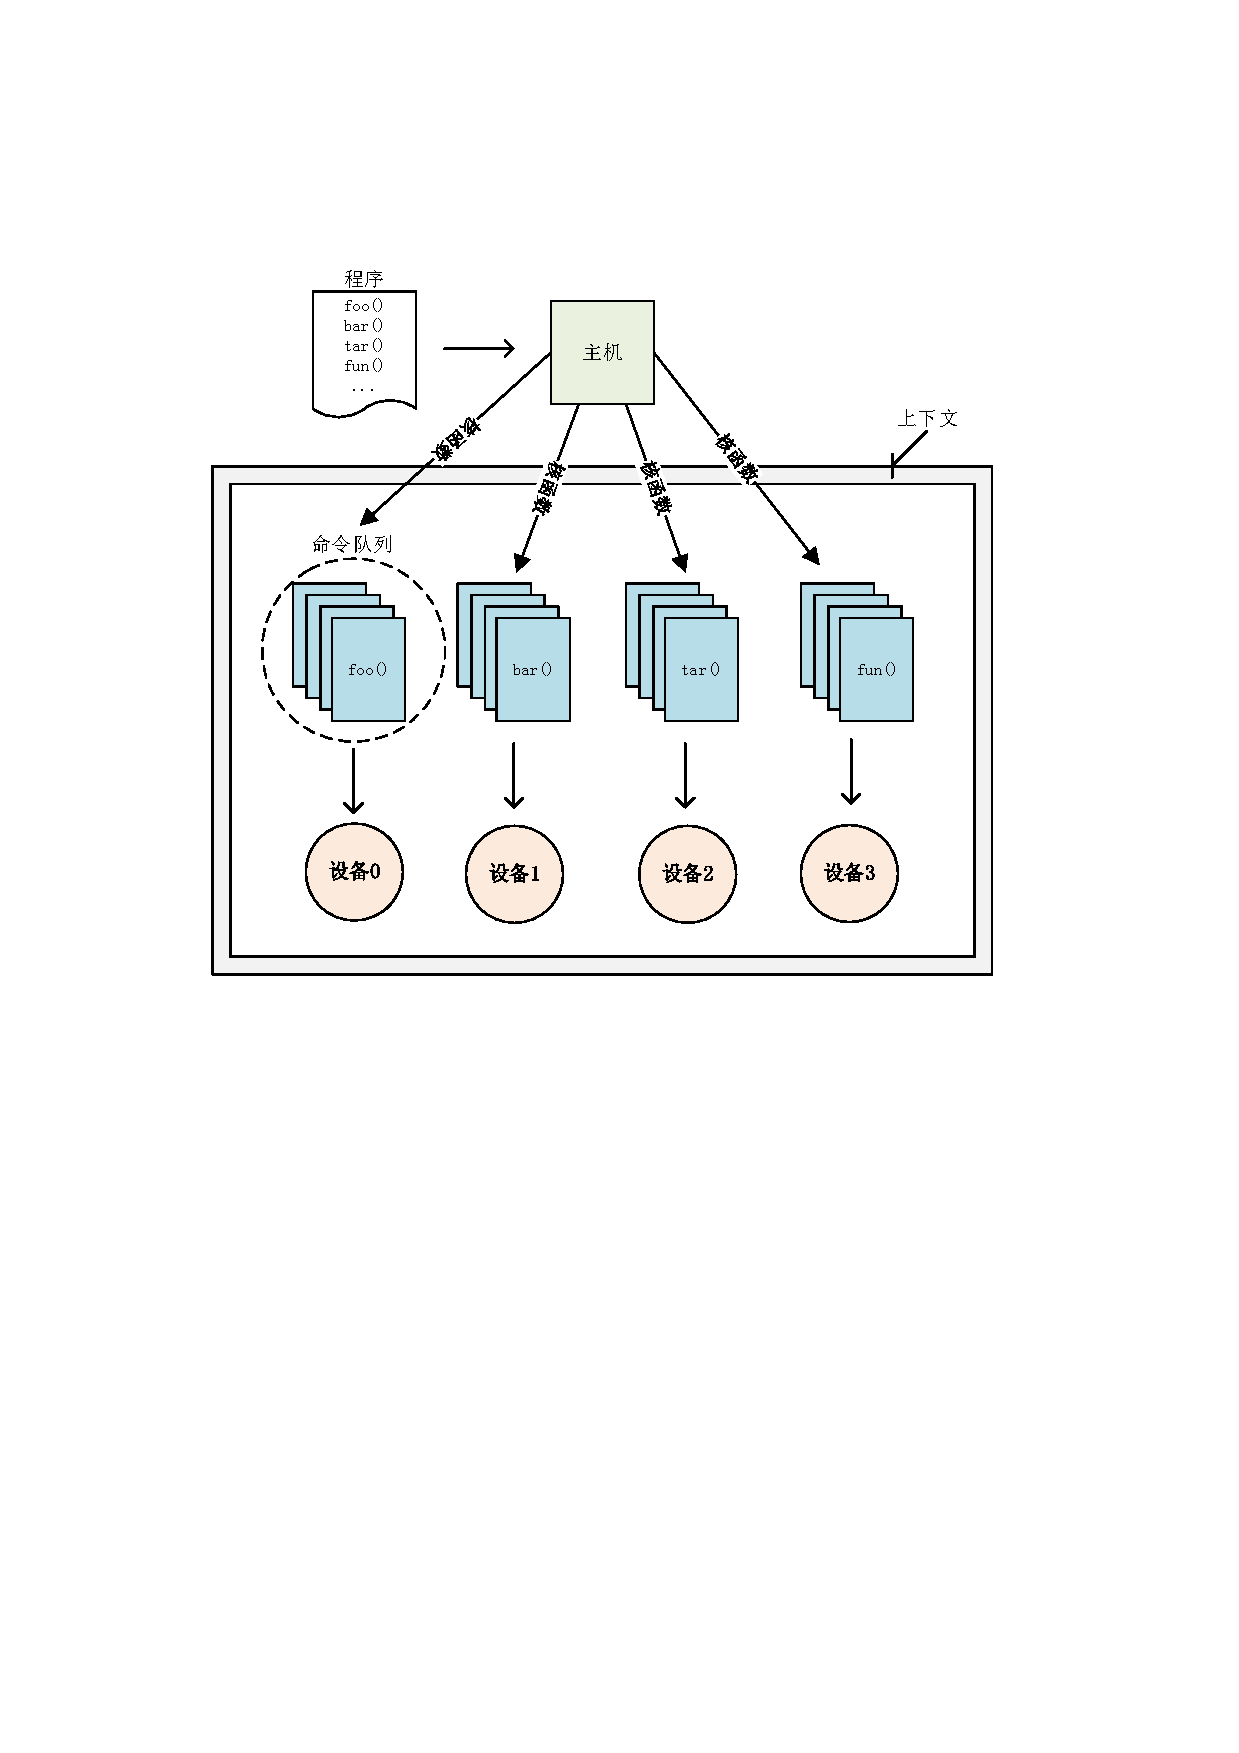
\includegraphics[width=0.8\textwidth, height=0.68\textwidth]{figures/opencl.pdf}
    \end{center}
    \caption{核函数在不同OpenCL兼容设备上的分发过程}\label{figure:figure7}
\end{figure}

OpenCL既支持数据并行操作,也提供完整的任务并行机制。换言之,OpenCL可在不同的处理单元上执行不同类型的计算任务。图\ref{figure:figure7}描述了OpenCL如何在不同的设备上完成任务并行逻辑。大多数的OpenCL设备拥有着不止一个的处理单元,这意味着在每个设备的内部还可以进行进一步的并行计算。

\subsection{OpenCL基本编程流程}

可移植性、向量处理以及并行编程使得OpenCL比常规的C/C++更加强大,但是使用OpenCL编写程序也比较复杂。下面给出OpenCL编程的基本流程:

\begin{enumerate}
  \item 访问OpenCL平台(\emph{platform})并选择所需平台。平台是由硬件厂商提供的OpenCL框架的具体实现,不同的异构硬件生产商(如Intel、AMD、Nvidia等)可以在一个系统上分别定义自己的OpenCL框架。故而在开发OpenCL程序前,程序设计者需要查询系统中可用的OpenCL框架实现。这就需要用到\emph{platform},其对应的数据结构是cl\_platform\_id。OpenCL框架定义的\texttt{clGetPlatformIDs()} API可以用来访问并获取可用的平台,通过API \texttt{clGetPlatformInfo()}可以查看与指定平台相关的信息。
  \item 访问指定平台上的设备并选择所需设备。通过厂商提供的平台,程序设计者可以访问每一个与之相连的设备。在OpenCL应用中,设备收到的任务和数据来源于主机。在代码中,设备由cl\_device\_id数据结构表示。查询并获得设备以及查看与特定设备相关的信息可分别通过OpenCL框架定义的\texttt{clGetDeviceIDs()}和\texttt{clGetDeviceInfo()}这两个API实现。
  \item 创建上下文并通过上下文管理设备。如前所述,OpenCL的上下文主要用来标识并管理一个设备集合。目前,一个上下文只能包含来自同一平台的设备,换言之,AMD和英伟达提供的设备不能放在同一个平台上。但是,主机应用可以通过创建多个上下文来管理不同厂商提供的设备,并且同一个平台上也可以创建多个上下文。创建上下文主要由\texttt{clCreateContext()}和\texttt{clCreateContextFromType()}两个API完成。
  \item 通过上下文创建命令队列。每个命令队列与特定的某个设备一一对应,主机应用可以通过命令队列对设备进行操作,如执行核函数、设置核函数参数以及读写设备内存等。默认地,命令队列按接收顺序执行命令,但是在创建命令时也可以改变这种默认行为。\texttt{clCreateCommandQueue()} API可完成命令队列的创建工作。
  \item 使用程序(\emph{program})存储设备代码。一个程序包含了许多核函数的实现代码,由数据结构cl\_program表示。程序设计人员可以将一个文本字符串通过 \texttt{clCreateProgramWithSource()} API转换为程序这种数据结构,并可使用API \texttt{clBuildProgram()}对创建的程序进行编译。因为OpenCL使用厂商提供的编译器对设备代码进行编译,所以编译信息需要使用API \texttt{clGetProgramBuildInfo()}得到。
  \item 从程序中提取核函数(\emph{kernel})。对程序进行编译、链接后,可以使用核函数这种数据结构(cl\_kernel)将每个函数功能进行封装。核函数可以被分发到一个命令队列,进而可被与该命令队列所关联的设备执行。通过API \texttt{clCreateKernel()}可对程序中的每一个函数进行核函数封装,而API \texttt{clGetKernelInfo()}可以用来查询指定核函数的相关信息。
  \item 设置核函数参数并执行核函数。程序设计人员可以使用\texttt{clEnqueueTask()}和\texttt{clEnqueueNDRangeKernel()}这两个API将核函数入列执行,而核函数的参数可以使用API \texttt{clSetKernelArg()}进行设置。核函数入列后并不意味着马上执行,其必须要在相应的命令队列中排队等待。
  \item 读取执行结果并释放OpenCL资源。OpenCL提供了许多以clEnqueue开头的API,每一个这种函数都是通过命令队列向设备发送命令。其中,可用来读取核函数执行结果的API包括\texttt{clEnqueueReadBuffer()} 和\texttt{clEnqueueMapBuffer()}。另外,凡是通过以clCreate开头的API创建的数据结构必须通过以clRelease开头的对应API进行资源的释放。
\end{enumerate}

\section{能效度量标准与实验平台}
\label{chapter:ch2-4}
本文使用\texttt{Energy Delay Product(EDP)}\cite{horowitz1994low}评估CNN前向推断过程中所涉及操作的执行能效,\ref{chapter:edp}节对$EDP$的概念以及选择原因进行了阐述。由于本文其他章节的实验部分都是基于ODROID-XU3\cite{hardkernel.com}和Open-Q™ 820\cite{intrinsyc.com}两个平台进行的,故而\ref{chapter:chapter2-5-1}节和\ref{chapter:chapter2-5-2}节分别对两个平台进行了详细介绍。

\subsection{能效度量标准}
\label{chapter:edp}

Energy Delay Product(EDP)是由Horowitz提出并被用于评估数字电路设计领域中电路级功耗节约技术提升的能效,之后又被Brooks推广使用\cite{brooks2000power}。现在,$EDP$也经常被用来评估给定某一程序的执行能效。本文主要使用$EDP$评估一个计算过程(如CNN前向推断)使用不同优化方法所达到的能效值,它反映了该计算过程的计算延迟时间和电池电量消耗之间的折中。因此,本文中$EDP$被定义为一个计算过程的所需执行时间与所消耗电量之积,用公式形式化如下:

\begin{equation}
     \label{equation:equation1}
     \begin{aligned}
        EDP = E \times T
     \end{aligned}
\end{equation}

\noindent 本文中,$E$代表某一计算过程的平均能耗,$T$代表某一计算过程的平均执行时间。很明显,$EDP$是一个值越小越好的度量标准。

除EDP可作为能效度量标准外,性能与功耗之比(Performance per Watt,PPW)、性能与能耗之比(Performance per Joule,PPJ)也经常被研究学者用于评估一个计算过程的执行能效。另一方面,在CNN前向推断过程中,每秒处理图像数据的帧数(Frame per Second,FPS\cite{wang2017building})经常作为CNN推断执行性能的度量标准。因此,在CNN前向推断过程中,性能与功耗之比可由公式\ref{equation:equationfps}和公式\ref{equation:equationppw}推理得到,而性能与能耗之比可由公式\ref{equation:equationfps}和公式\ref{equation:equationppj}推理得到。三个公式中,$T$代表执行时间,$P$代表平均功耗,$E$代表能耗。

\begin{equation}
     \label{equation:equationfps}
     \begin{aligned}
        FPS = \frac{1}{T}
     \end{aligned}
\end{equation}

\begin{equation}
     \label{equation:equationppw}
     \begin{aligned}
        PPW = \frac{FPS}{P}
        = \frac{\frac{1}{T}}{P}
        = \frac{1}{P \times T}
        = \frac{1}{E}
     \end{aligned}
\end{equation}

\begin{equation}
     \label{equation:equationppj}
     \begin{aligned}
        PPJ = \frac{FPS}{E}
        = \frac{\frac{1}{T}}{E}
        = \frac{1}{E \times T}
        = \frac{1}{EDP}
     \end{aligned}
\end{equation}

根据公式\ref{equation:equationppw}可知,在CNN前向推断过程中,性能与功耗之比即为能耗的倒数。因此,性能与功耗之比仅仅强调了CNN前向推断的能耗因素,不能够全面反映推断过程的性能和能耗折中。根据公式\ref{equation:equationppj}可知,在CNN前向推断过程中,性能与能耗之比即为$EDP$的倒数,其为一个值越大越好的度量标准。无论是选择性能与能耗之比还是$EDP$,度量能效的结果都是一致的。故而,本文最终选用$EDP$作为CNN前向推断过程中所涉及计算执行能效的度量标准。

\subsection{ODROID-XU3}
\label{chapter:chapter2-5-1}
图\ref{figure:figureodroid}所示即为Hardkernel公司生产的ODROID-XU3开发平台,其采用三星\texttt{Exynos5422}作为SoC(内部集成2GB内存和\texttt{ARM Mali-T628 MP6} GPU)。实验中,ODROID-XU3运行的操作系统为Android 5.1.1版本(内核版本号为3.10.9)。\texttt{Exynos5422}的处理器使用了ARM的big.LITTLE\cite{chung2012heterogeneous}技术,并由四个\texttt{ARM Cortex-A15}大核(频率最高可达2.0GHz)和四个\texttt{ARM Cortex-A7}小核(频率最高可达1.4GHz)组成。由于使用了\texttt{big.LITTLE™ HMP}解决方案,\texttt{Exynos5422}最多可以使用8个核去处理计算密集型的任务。\texttt{ARM Mali-T628 MP6} GPU拥有两个GPU簇,即GPU簇0包含4个\texttt{ARM Mali-T628}核而GPU簇1包含2个\texttt{ARM Mali-T628}核\cite{lokhmotov2015gemmbench}。故而,对于ODROID-XU3来说,所有可获得的本地设备处理器包括一个CPU设备和两个GPU设备\label{chapter:chapter1-1}。

\begin{figure}[htbp]
    \begin{center}
    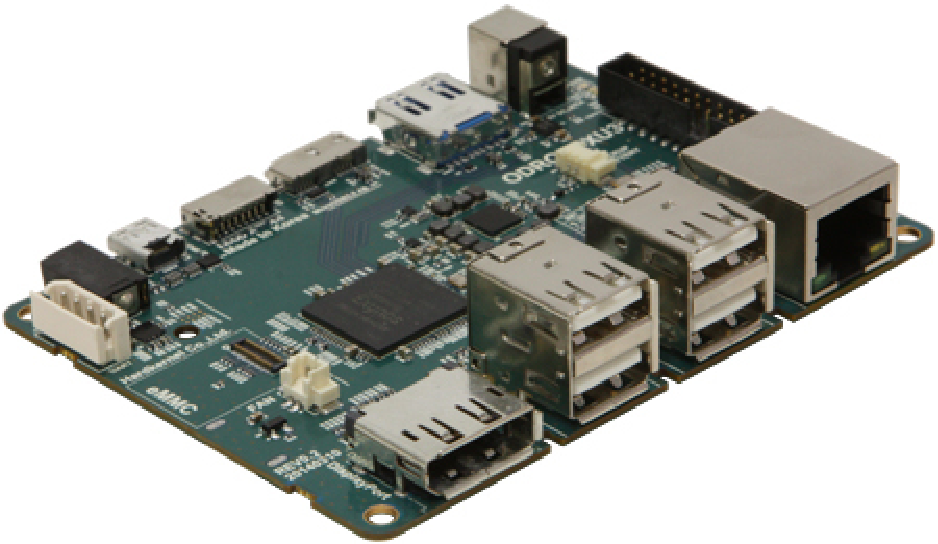
\includegraphics[width=0.5\textwidth]{figures/odroid.pdf}
    \end{center}
    \caption{ODROID-XU3}\label{figure:figureodroid}
\end{figure}

为了方便研究人员测量功耗和能耗,ODROID-XU3开发平台集成了4路电流/电压传感器,它们可以独立地测量大核A15、小核A7、GPU和内存(DRAMs)的实时功耗。因为Hardkernel公司官网并未提供Android平台使用传感器测量不同部件功耗或能耗的APP,而本文的实验部分却都是基于Android平台的,所以本文基于Android NDK开发了两个APP,即Power Monitor和Energy Update Service。它们可以分别用于测量给定程序某段运行过程的功耗(Power Monitor)和能耗(Energy Update Service)。

\begin{figure*}[htbp]
\centering
\subfigure[Power Monitor运行界面]{\label{subfig:subfigpower}
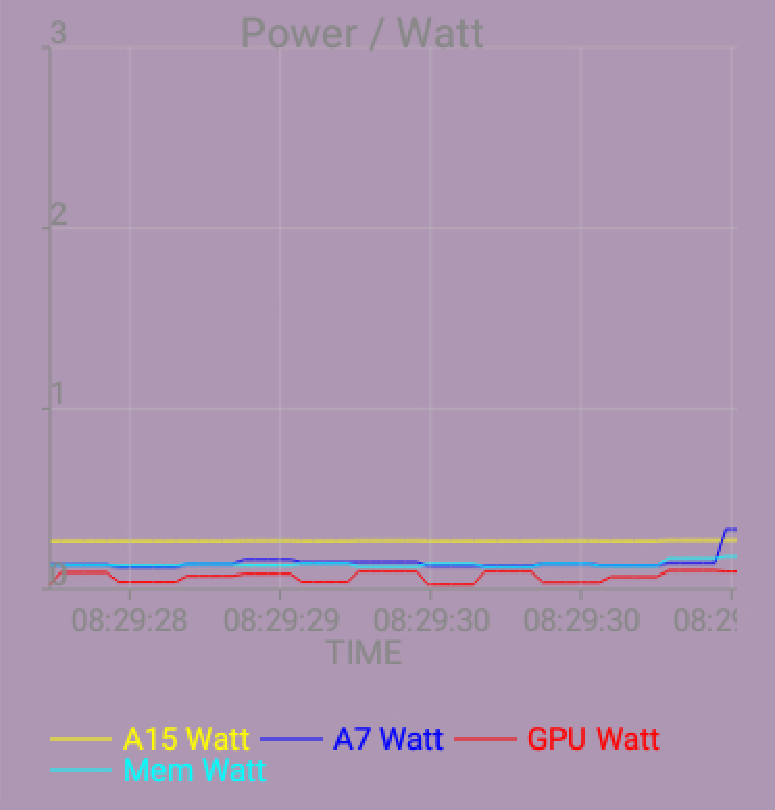
\includegraphics[scale=0.451]{figures/power.pdf}}
\subfigure[Energy Update Service运行界面]{\label{subfig:subfigenergy}
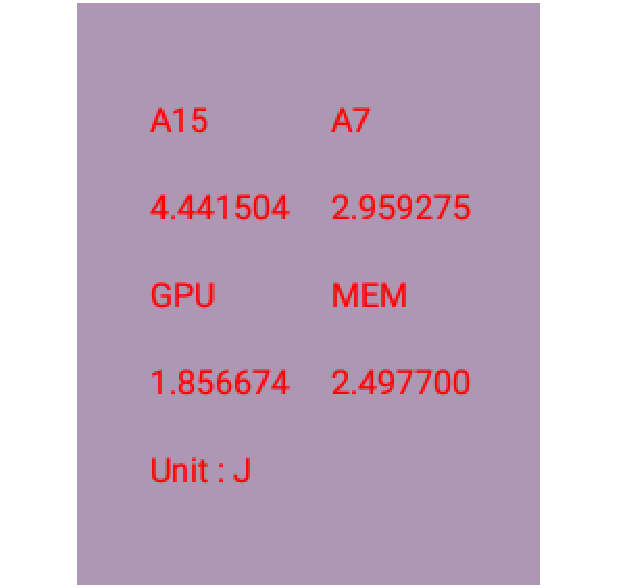
\includegraphics[scale=0.627]{figures/energy.pdf}}
\caption{功耗和能耗测量APP运行界面}
\label{fig:subfig}
\end{figure*}

\begin{itemize}
  \item \textbf{Power Monitor APP工作原理}:后台服务每隔50毫秒读取四路传感器的更新值,并将这些更新值追加到Power.csv文件中;前端浮动窗口每隔50毫秒进行一次界面刷新,并利用后台服务不断传回的四个传感器值绘制大核A15、小核A7、GPU和内存的实时功耗曲线。另外,实验中也可以选择关闭前端的浮动窗口以排除其能耗开销的干扰。浮动窗口关闭后,后台服务会继续运行以不断更新Power.csv的文件内容。之后,可以通过离线分析Power.csv的内容得到给定APP的功耗特征。Power Monitor的运行界面如图\ref{subfig:subfigpower}所示。
  \item \textbf{Energy Update Service APP工作原理}:后台服务每隔50毫秒读取四路传感器的更新值,并利用这些更新值求取自Energy Update Service应用启动以来大核A15、小核A7、GPU和内存的累积能耗。实验中系统内核经过修改加入了两个系统调用功能:380号系统调用用于将4个最新的累积能耗值(分别对应大核A15、小核A7、GPU和内存的累积能耗)更新到指定的内核空间,而381号系统调用用于随时读取该指定内核空间的四个累积能耗值。380号系统调用主要被后台服务用于将4个最新求取的累积能耗值更新至指定的内核空间(更新周期为50毫秒)。而其他Android应用只需在待测量功耗的代码段前后打上两个桩,通过两次执行381号系统调用即可得到运行前后的两个累积能耗值,两值之差即为运行该段代码所需的能耗。Energy Update Service应用的前端浮动窗口用于实时显示4个当前累积能耗值,其也可以被关闭且不会影响后台服务的正常运行。Energy Update Service的运行界面如图\ref{subfig:subfigenergy}所示。
\end{itemize}

\subsection{Open-Q™ 820开发套件}
\label{chapter:chapter2-5-2}

如图\ref{figure:figureopenQ}所示,Open-Q™ 820是Intrinsyc公司推出的一款基于骁龙820芯片的开发套件。骁龙820芯片不仅使用了四个主频可达2.2GHz的64位ARMv8核(\texttt{Kryo}),还配备了高通\texttt{Adreno 530} GPU和\texttt{Hexagon 680} DSP。其中,\texttt{Adreno 530} GPU虽然只包含了4个核心,但是性能要比\texttt{ARM Mali-T628 MP6} GPU强大许多。另外,Open-Q™ 820还配有3GB的\texttt{LPDDR4}板载内存。实验中,Open-Q™ 820运行的Android系统版本为7.0(代号为Android N),内核版本号为3.18.31。

\begin{figure}[htbp]
    \begin{center}
    \includegraphics[width=0.4\textwidth, height=0.4\textwidth]{figures/openQ.pdf}
    \end{center}
    \caption{Open-Q™ 820开发套件}\label{figure:figureopenQ}
\end{figure}

本文的实验部分主要基于ODROID-XU3开发平台展开,这是因为使用本文所开发的Power Monitor和Energy Update Service两款Android应用可以很容易地在ODROID-XU3平台上获取一段程序执行过程所产生的能耗和功耗。Open-Q™ 820开发套件主要用于验证本文所开发CNN推断时库的可移植性和兼容性,并与ODROID-XU3开发平台的CNN推断执行性能做对比。

\section{本章小结}

本章首先介绍了卷积神经网络的概念和其中一些基本层的含义与作用,这为下一章分解卷积神经网络前向推断过程中的基本算子做足了准备。因为本研究工作中使用“剪枝-重训”方法对卷积神经网络的权重进行压缩,故而本章对深度学习模型训练过程中所使用的反向传播算法进行了详细描述。另外,\ref{chapter:chapteropencl}节对本研究中所使用的异构编程框架OpenCL的基本概念及其具备的三个主要优点进行了介绍,并给出了开发基于OpenCL的异构程序的基本编程流程。最后,本章对研究中所使用的能效评估度量标准以及实验平台进行了详细说明。

\cleardoublepage 